% !TEX root = ../rawlik-phd-thesis.tex
\chapter{SFC prototype}
\label{ch:sfc-prototype}

Short introduction and overview\ldots
The goal was do demonstrate the feasibility of construction of the coils, develop and test the electronic and software parts of the feedback algorithm, and test the whole system.

It is based on the coil design method described earlier.


\section{The first iteration}
Start by describing the support structure. In the cable channels many coils may be laid. A structure was build. Some technical details: Item profiles, cut aluminum plates.

\begin{figure}
  \centering
  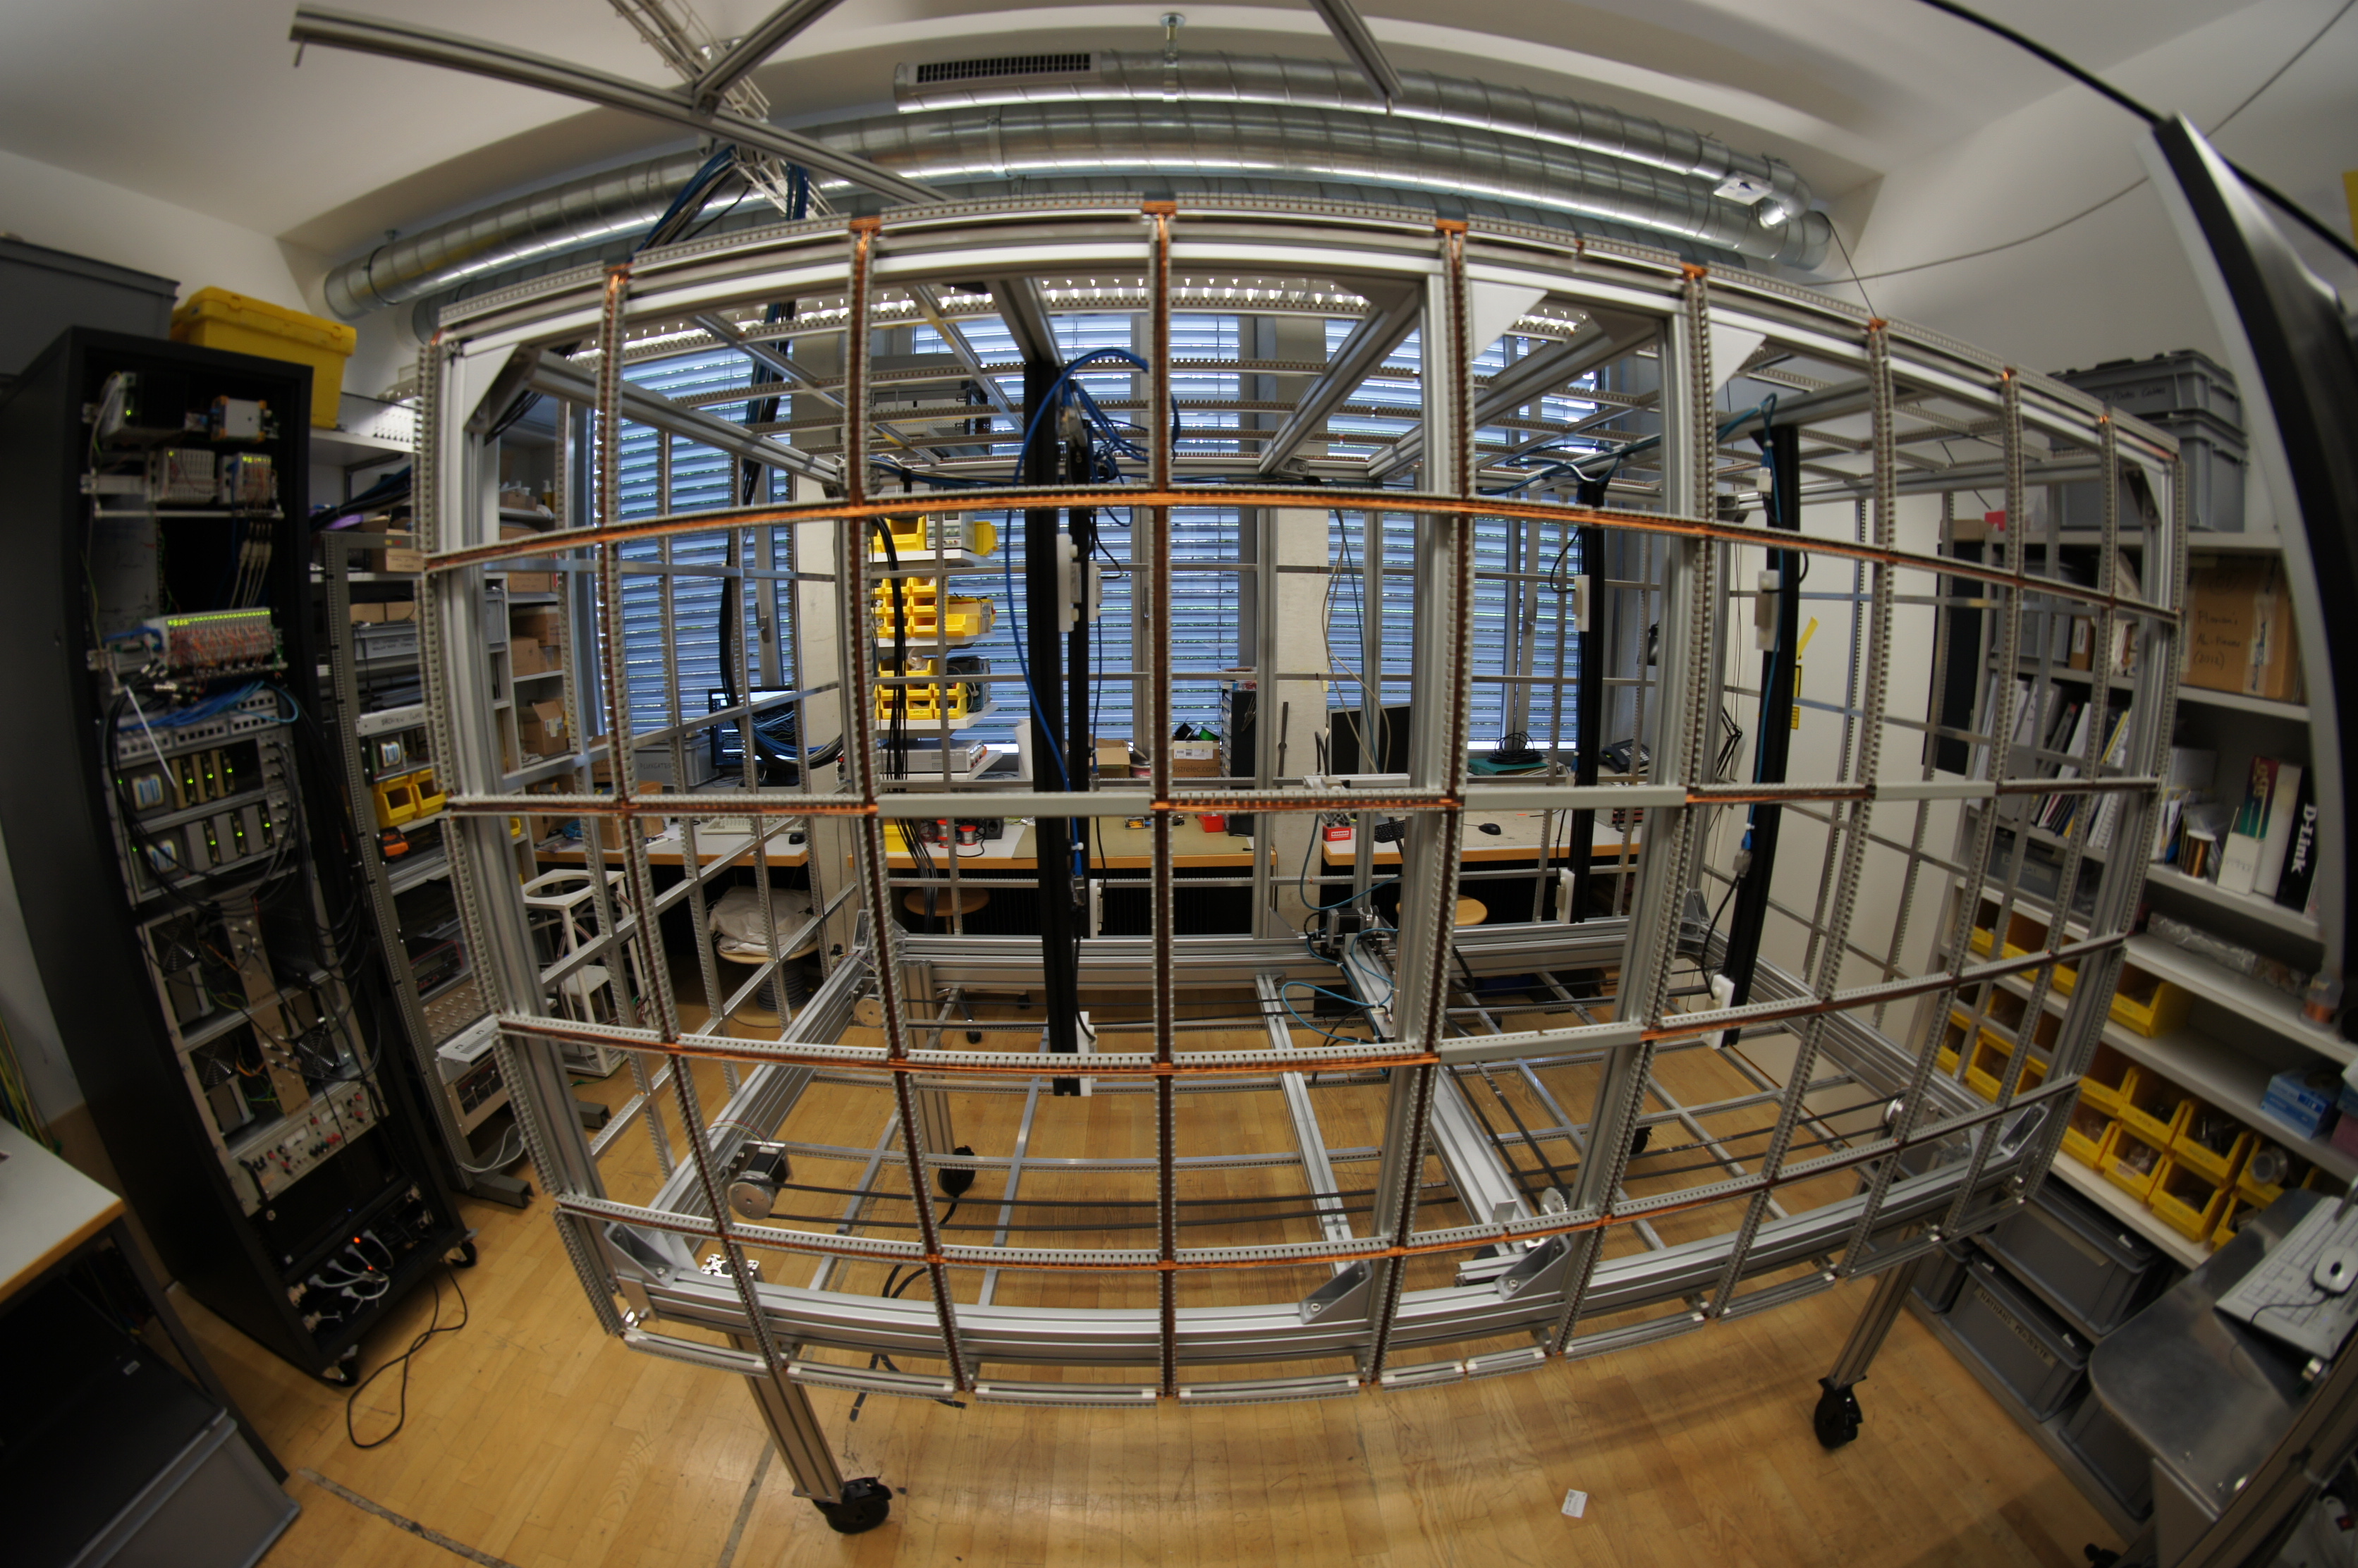
\includegraphics[width=0.9\linewidth]{gfx/prototype/DSC03472.JPG}
  \caption{Mention, that it shows\ldots}
  \label{fig:prototype_photo}
\end{figure}

\begin{figure}
  \centering
  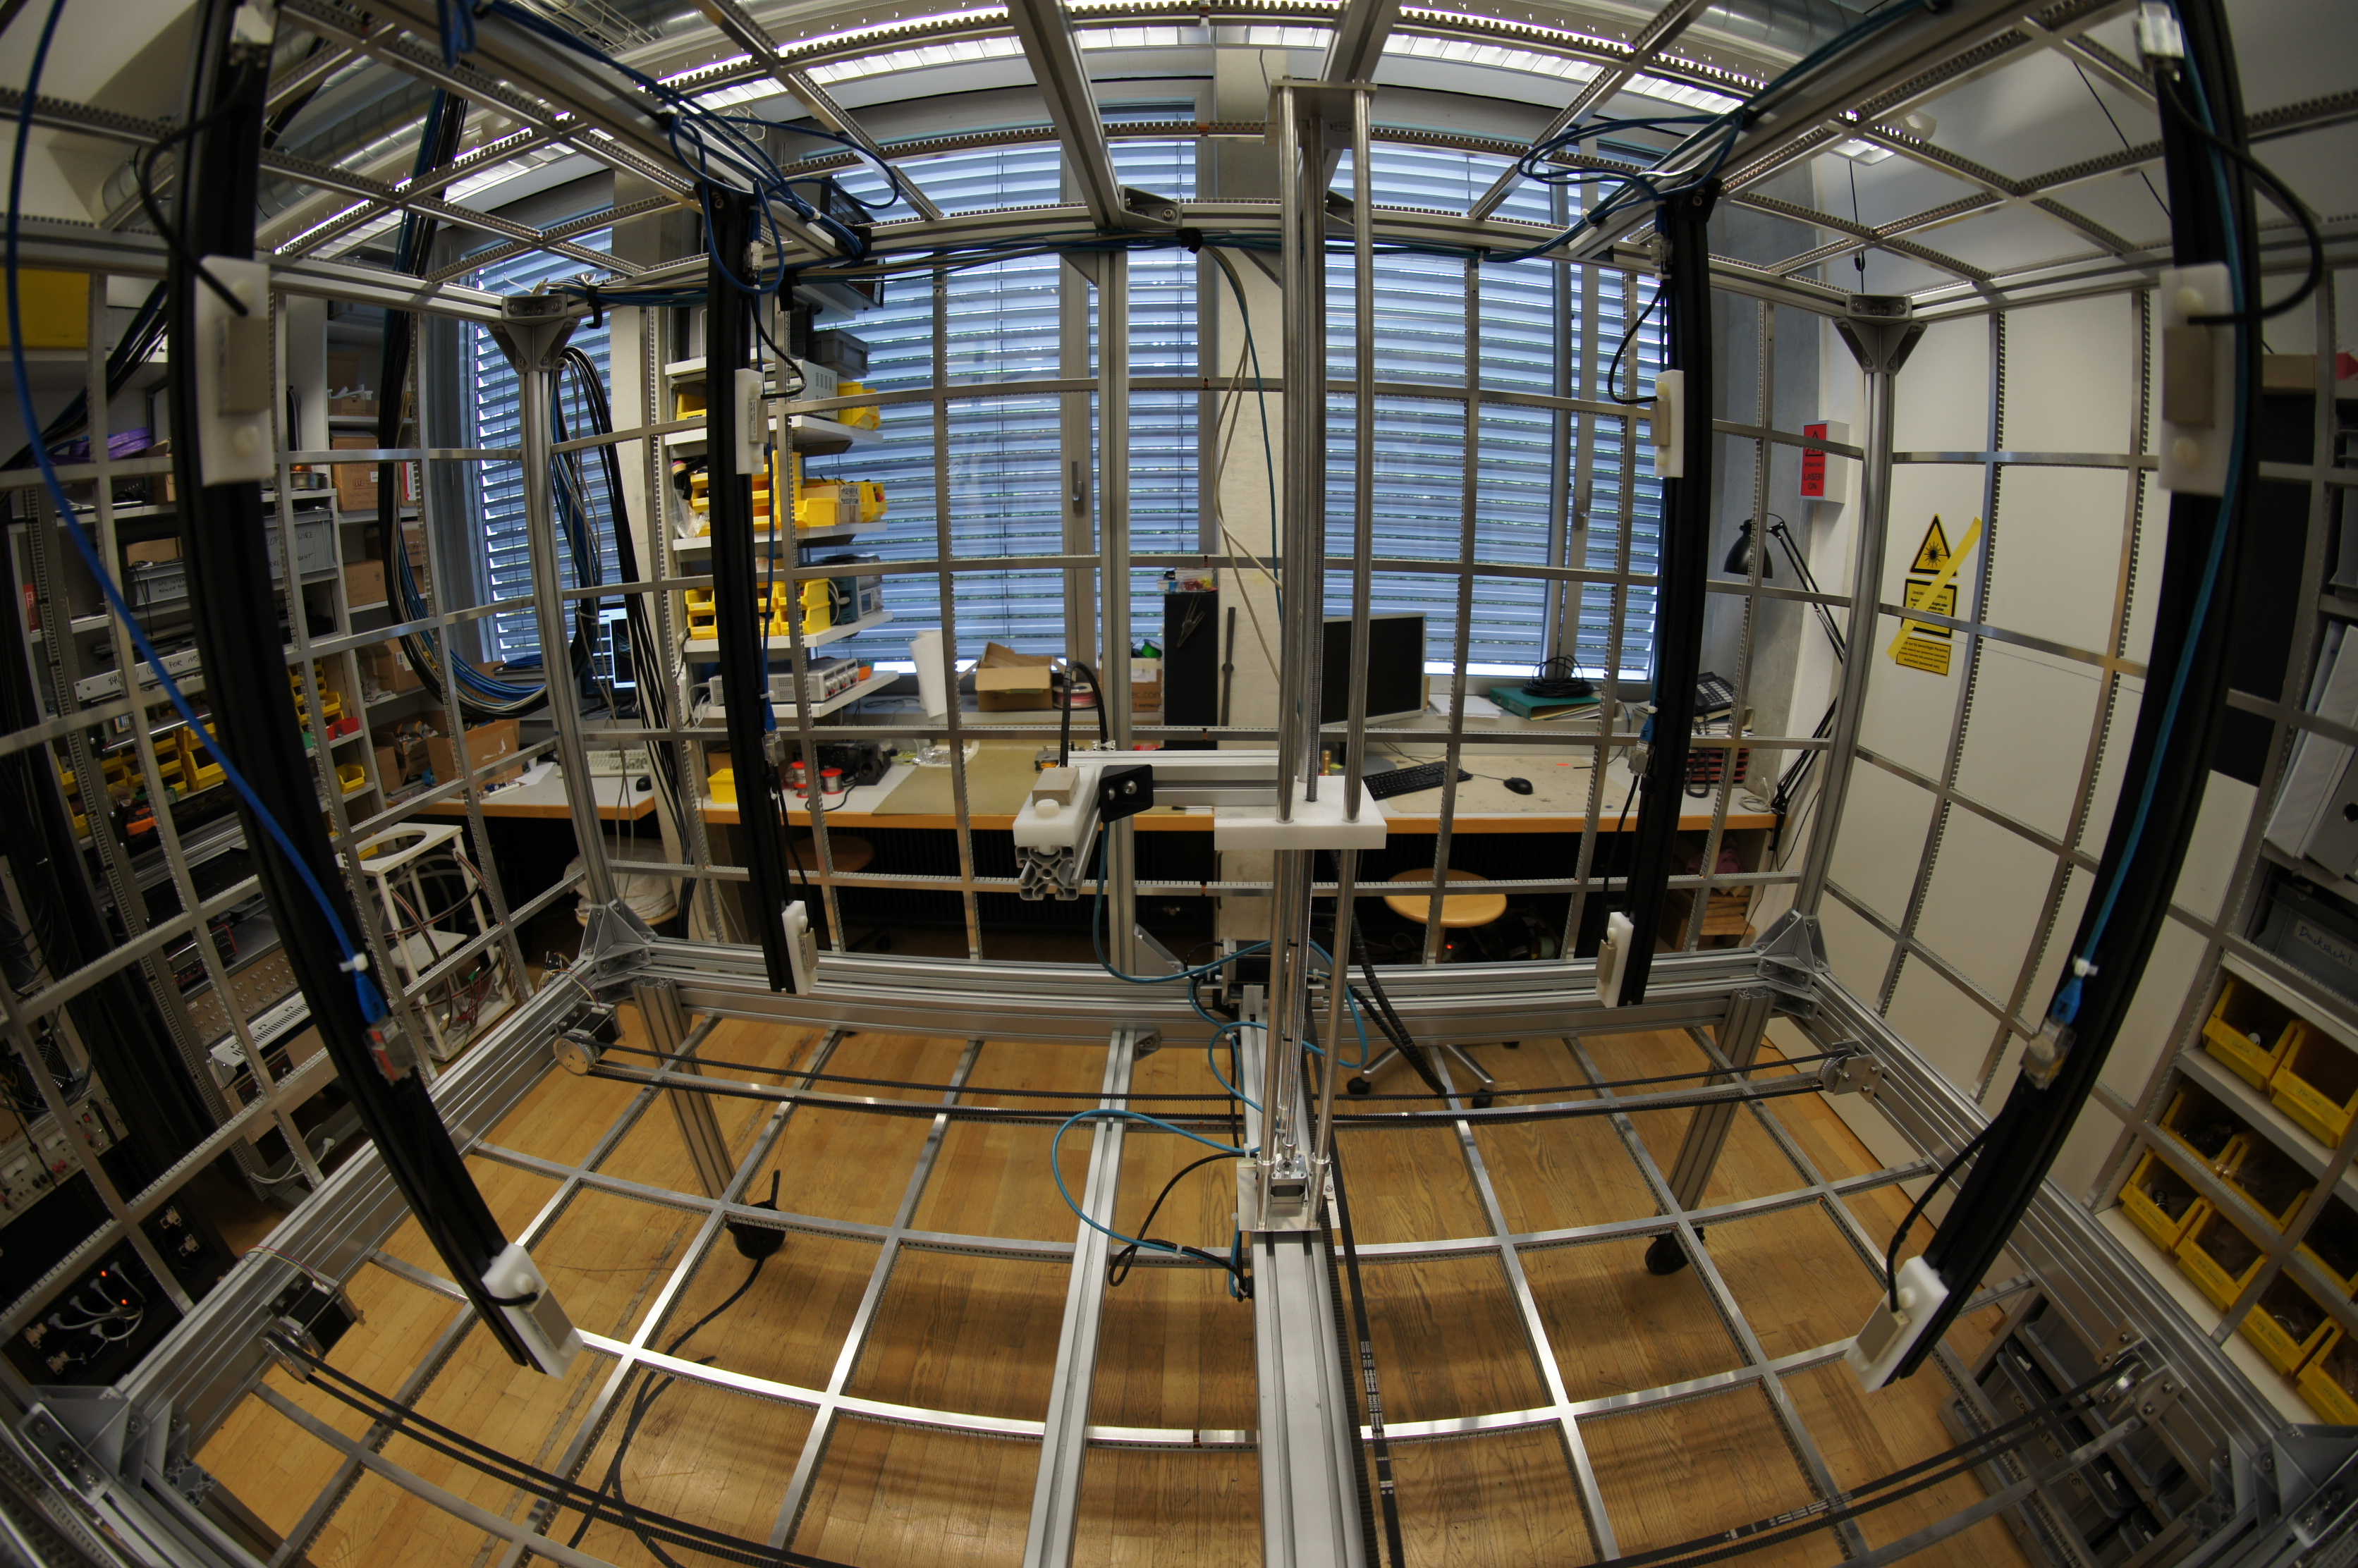
\includegraphics[width=0.9\linewidth]{gfx/prototype/DSC03476.JPG}
  \caption{Mention, that it shows\ldots}
  \label{fig:prototype_photo_inside}
\end{figure}

\begin{figure}
  \centering
  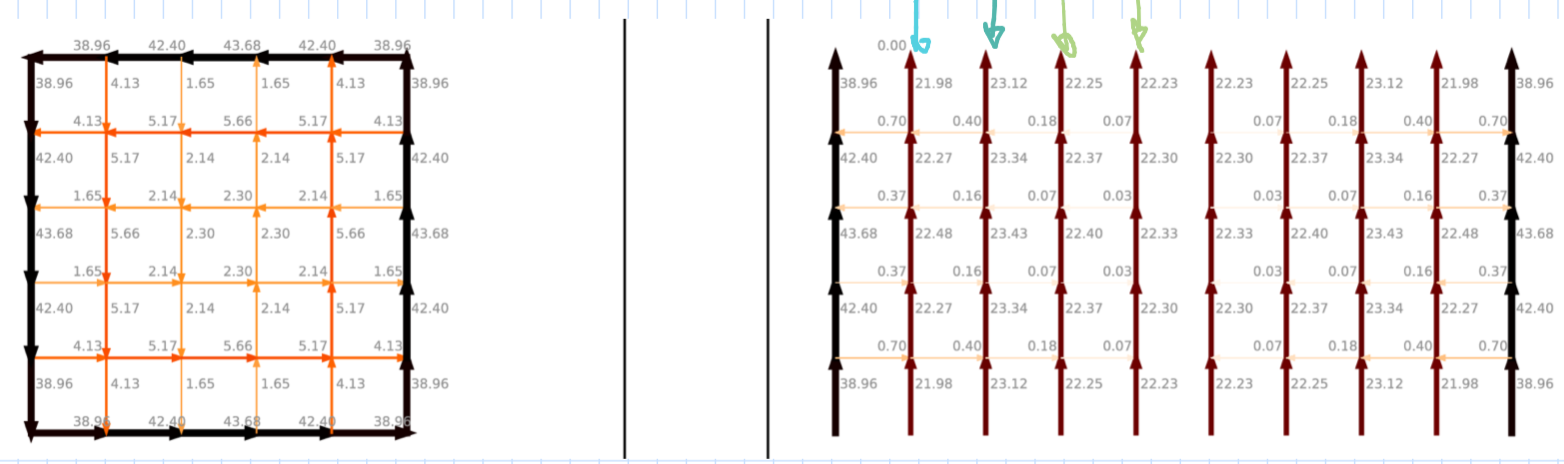
\includegraphics[width=0.9\linewidth]{gfx/prototype/coil_y_currents.png}
  \caption{Mention, that it shows\ldots}
  \label{fig:prototype_coil_y_currents}
\end{figure}

\begin{figure}
  \centering
  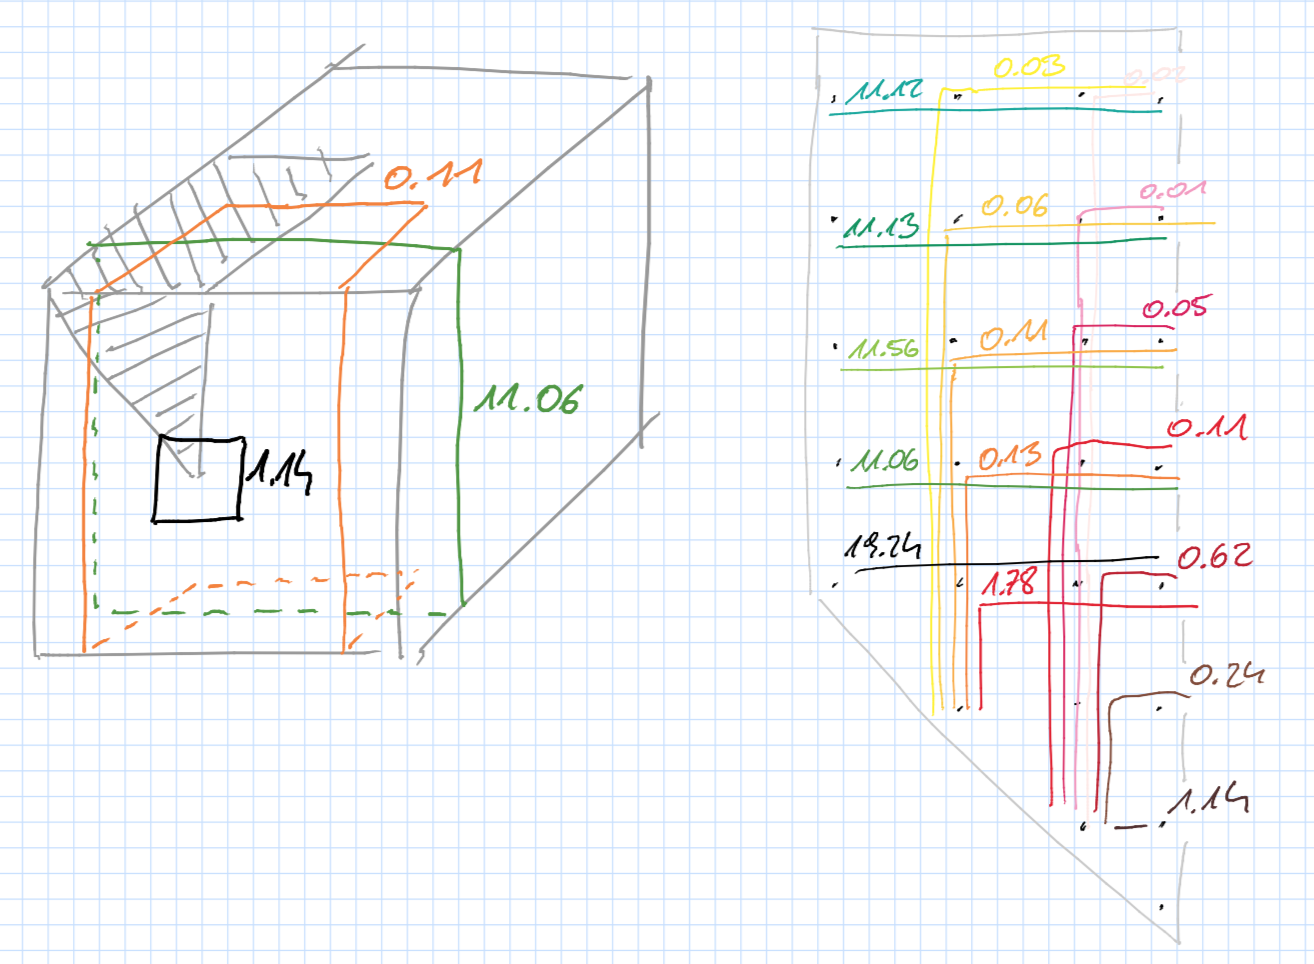
\includegraphics[width=0.9\linewidth]{gfx/prototype/coil_y_decomposition.png}
  \caption{Mention, that it shows\ldots}
  \label{fig:prototype_coil_y_decomposition}
\end{figure}

\begin{figure}
  \centering
  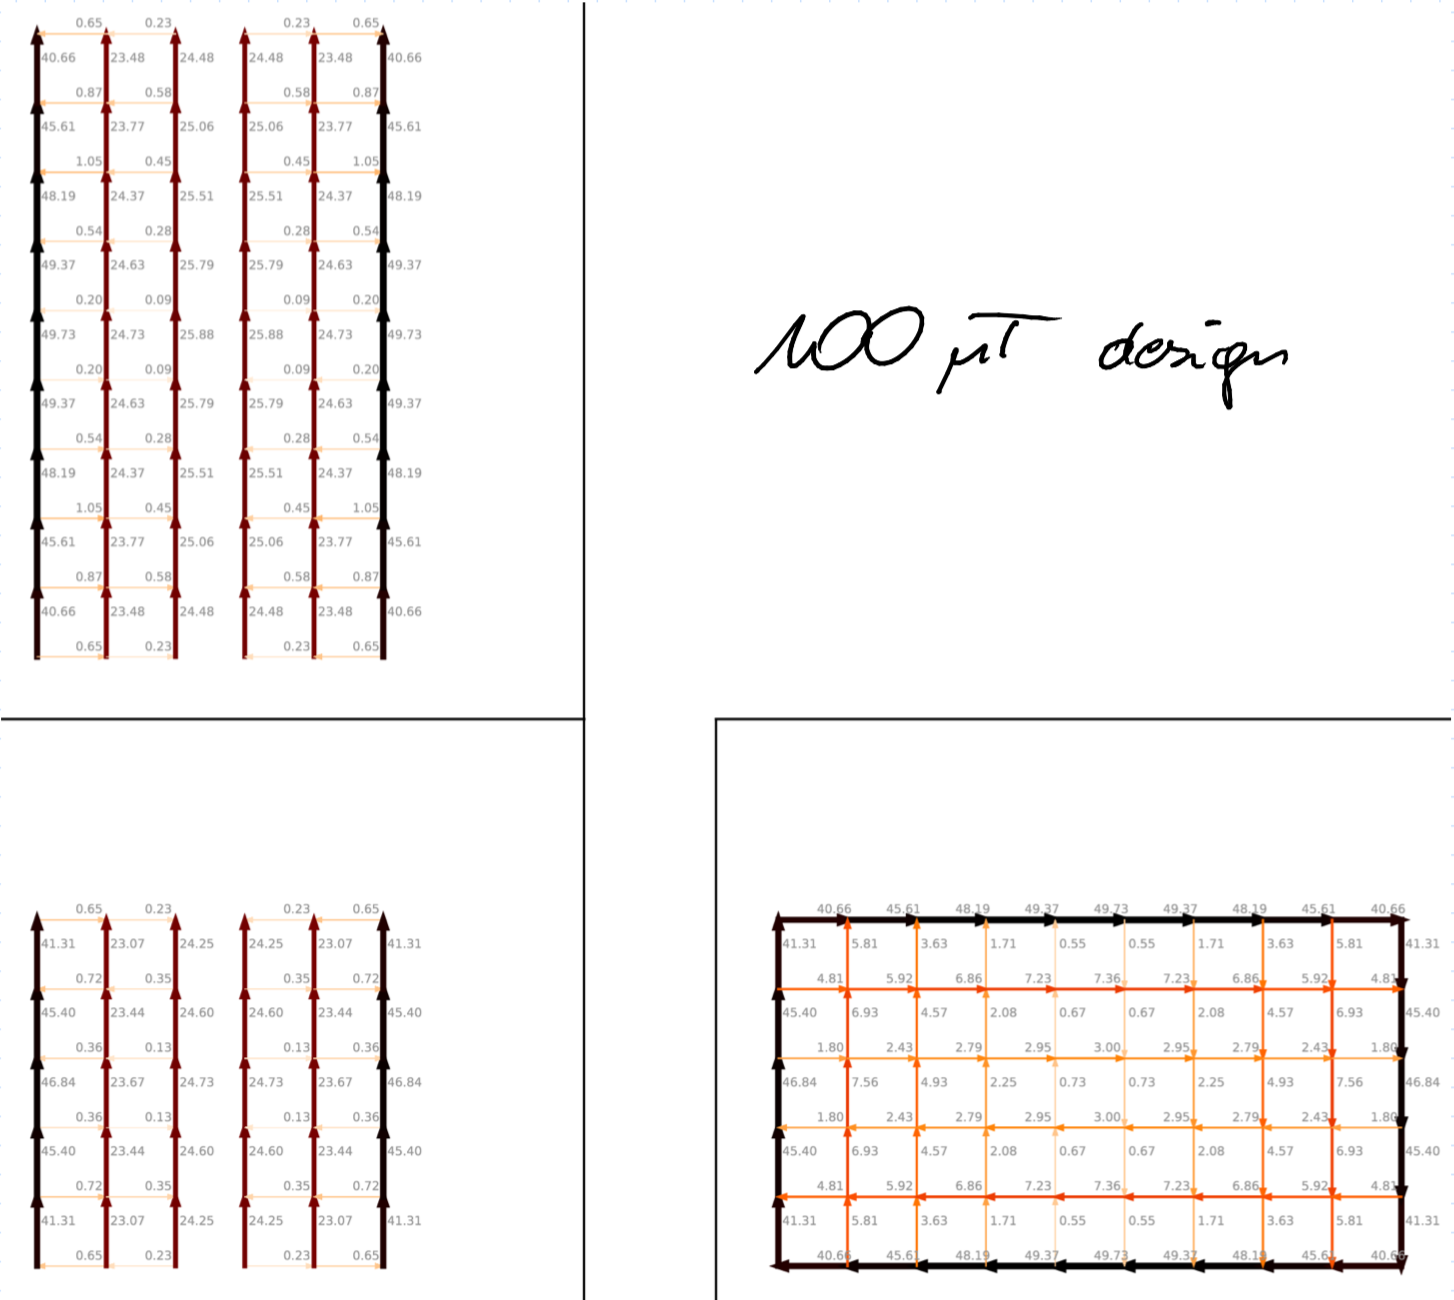
\includegraphics[width=0.9\linewidth]{gfx/prototype/coil_x_z_currents.png}
  \caption{Mention, that it shows\ldots}
  \label{fig:prototype_coil_x_z_currents}
\end{figure}

\begin{figure}
  \centering
  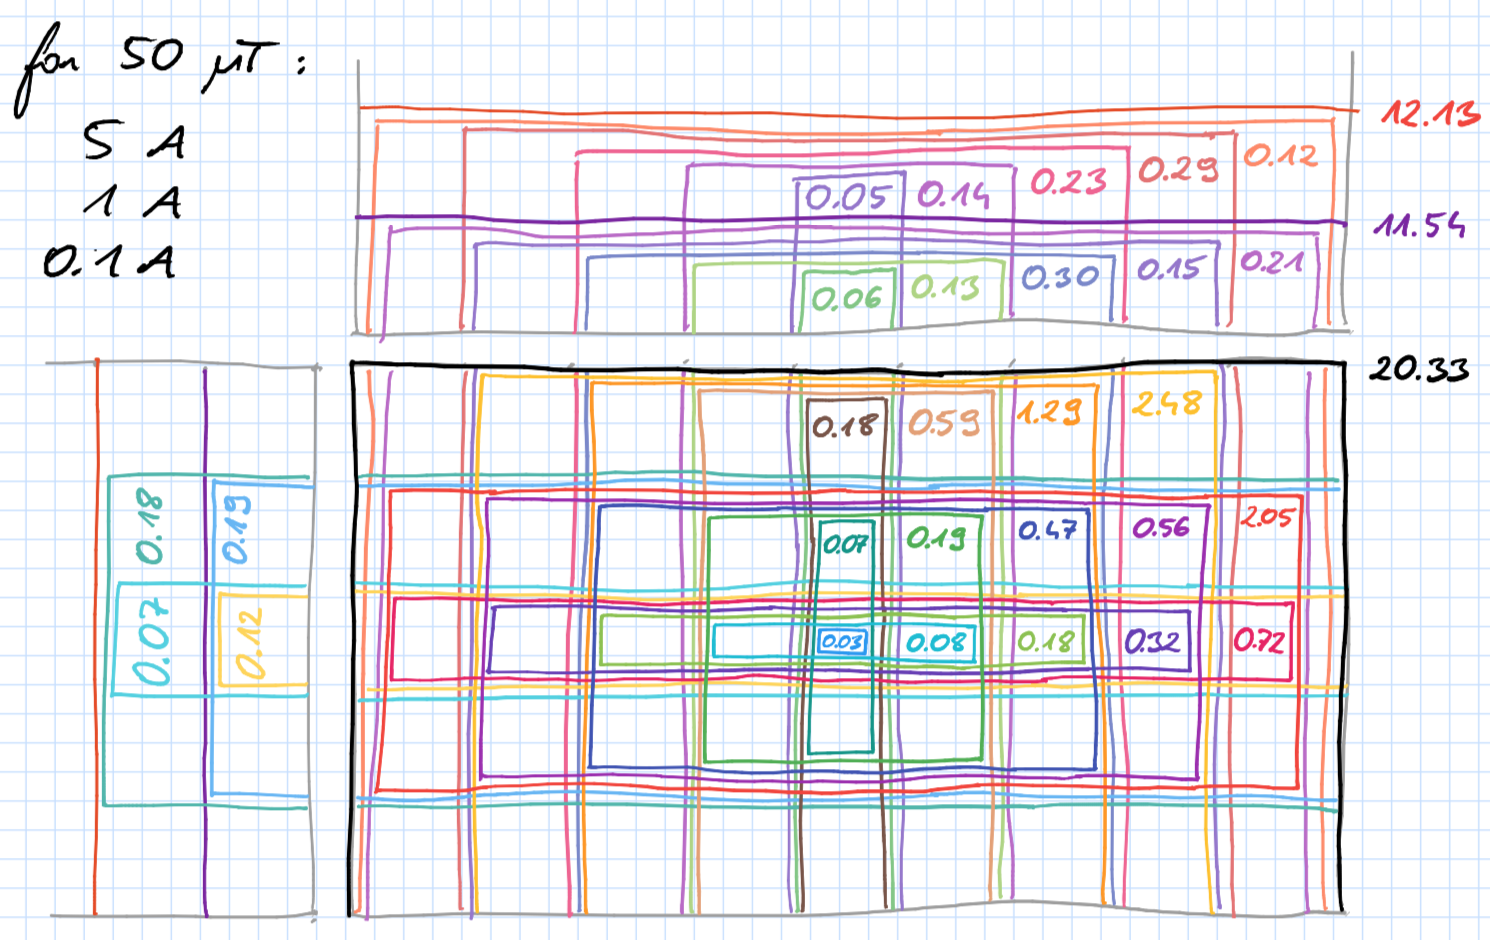
\includegraphics[width=0.9\linewidth]{gfx/prototype/coil_x_z_decomposition.png}
  \caption{Mention, that it shows\ldots}
  \label{fig:prototype_coil_x_z_decomposition}
\end{figure}

The first iteration of the prototype had 3 coils for the homogeneous field

\begin{figure}
  \centering
  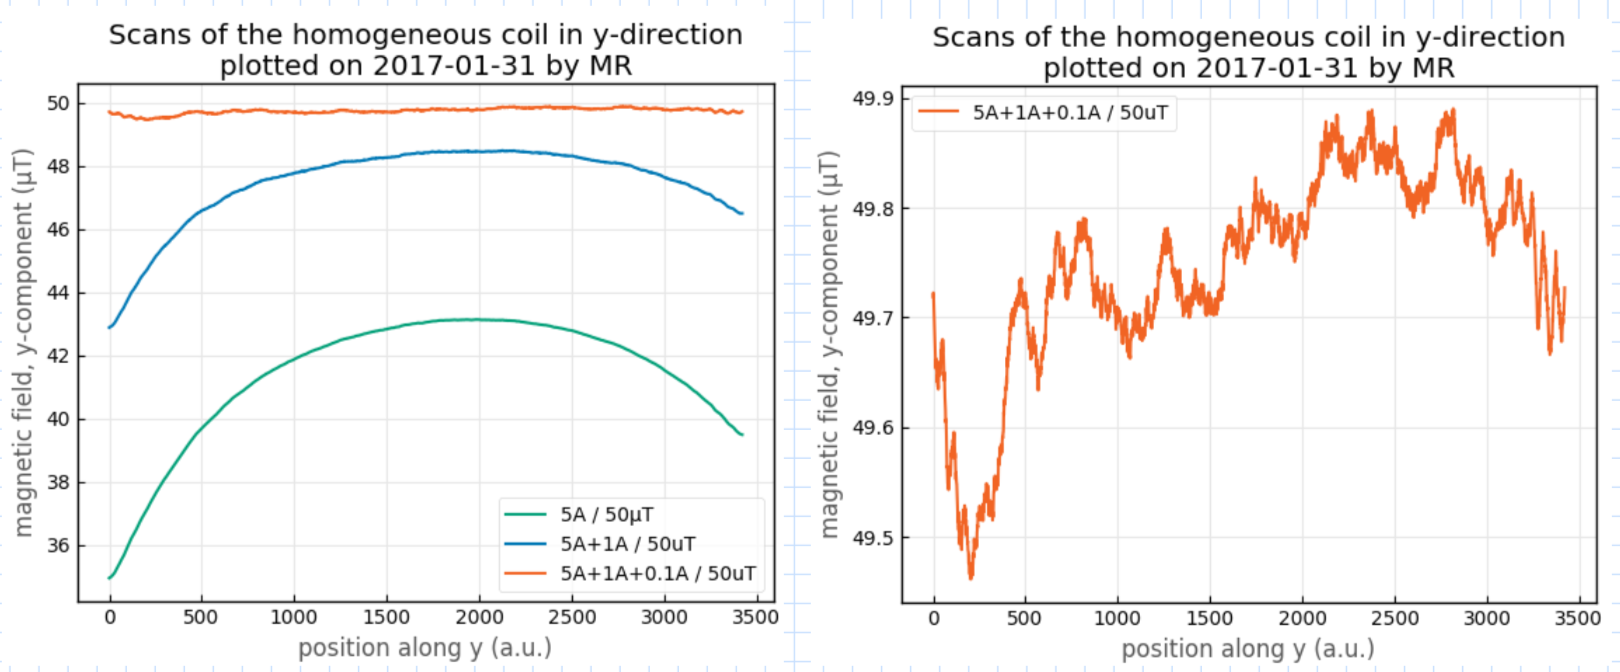
\includegraphics[width=0.9\linewidth]{gfx/prototype/linear_map.png}
  \caption{Mention, that it shows\ldots}
  \label{fig:prototype_linear_map}
\end{figure}

\begin{figure}
  \centering
  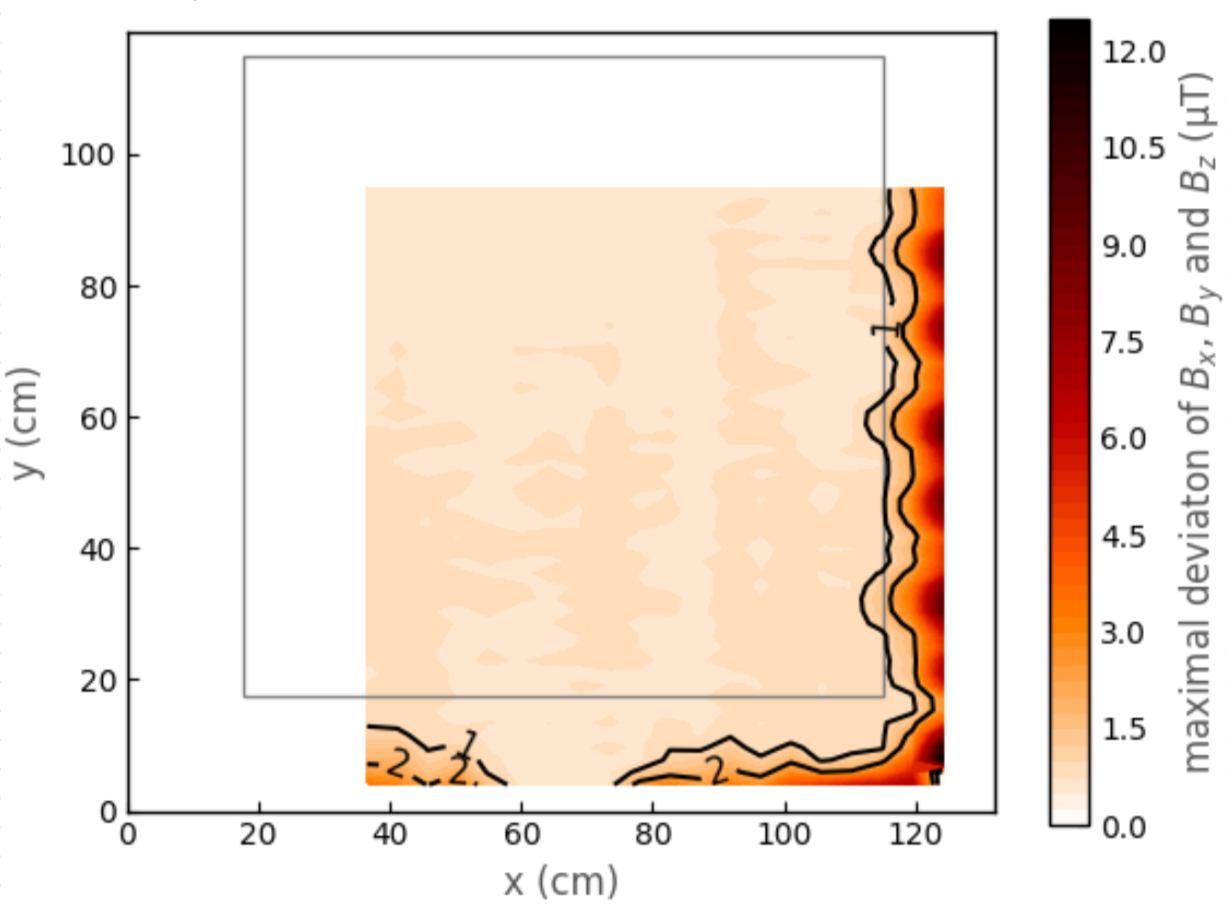
\includegraphics[width=0.9\linewidth]{gfx/prototype/plane_map.png}
  \caption{Mention, that it shows\ldots}
  \label{fig:prototype_plane_map}
\end{figure}


\begin{figure}
  \centering
  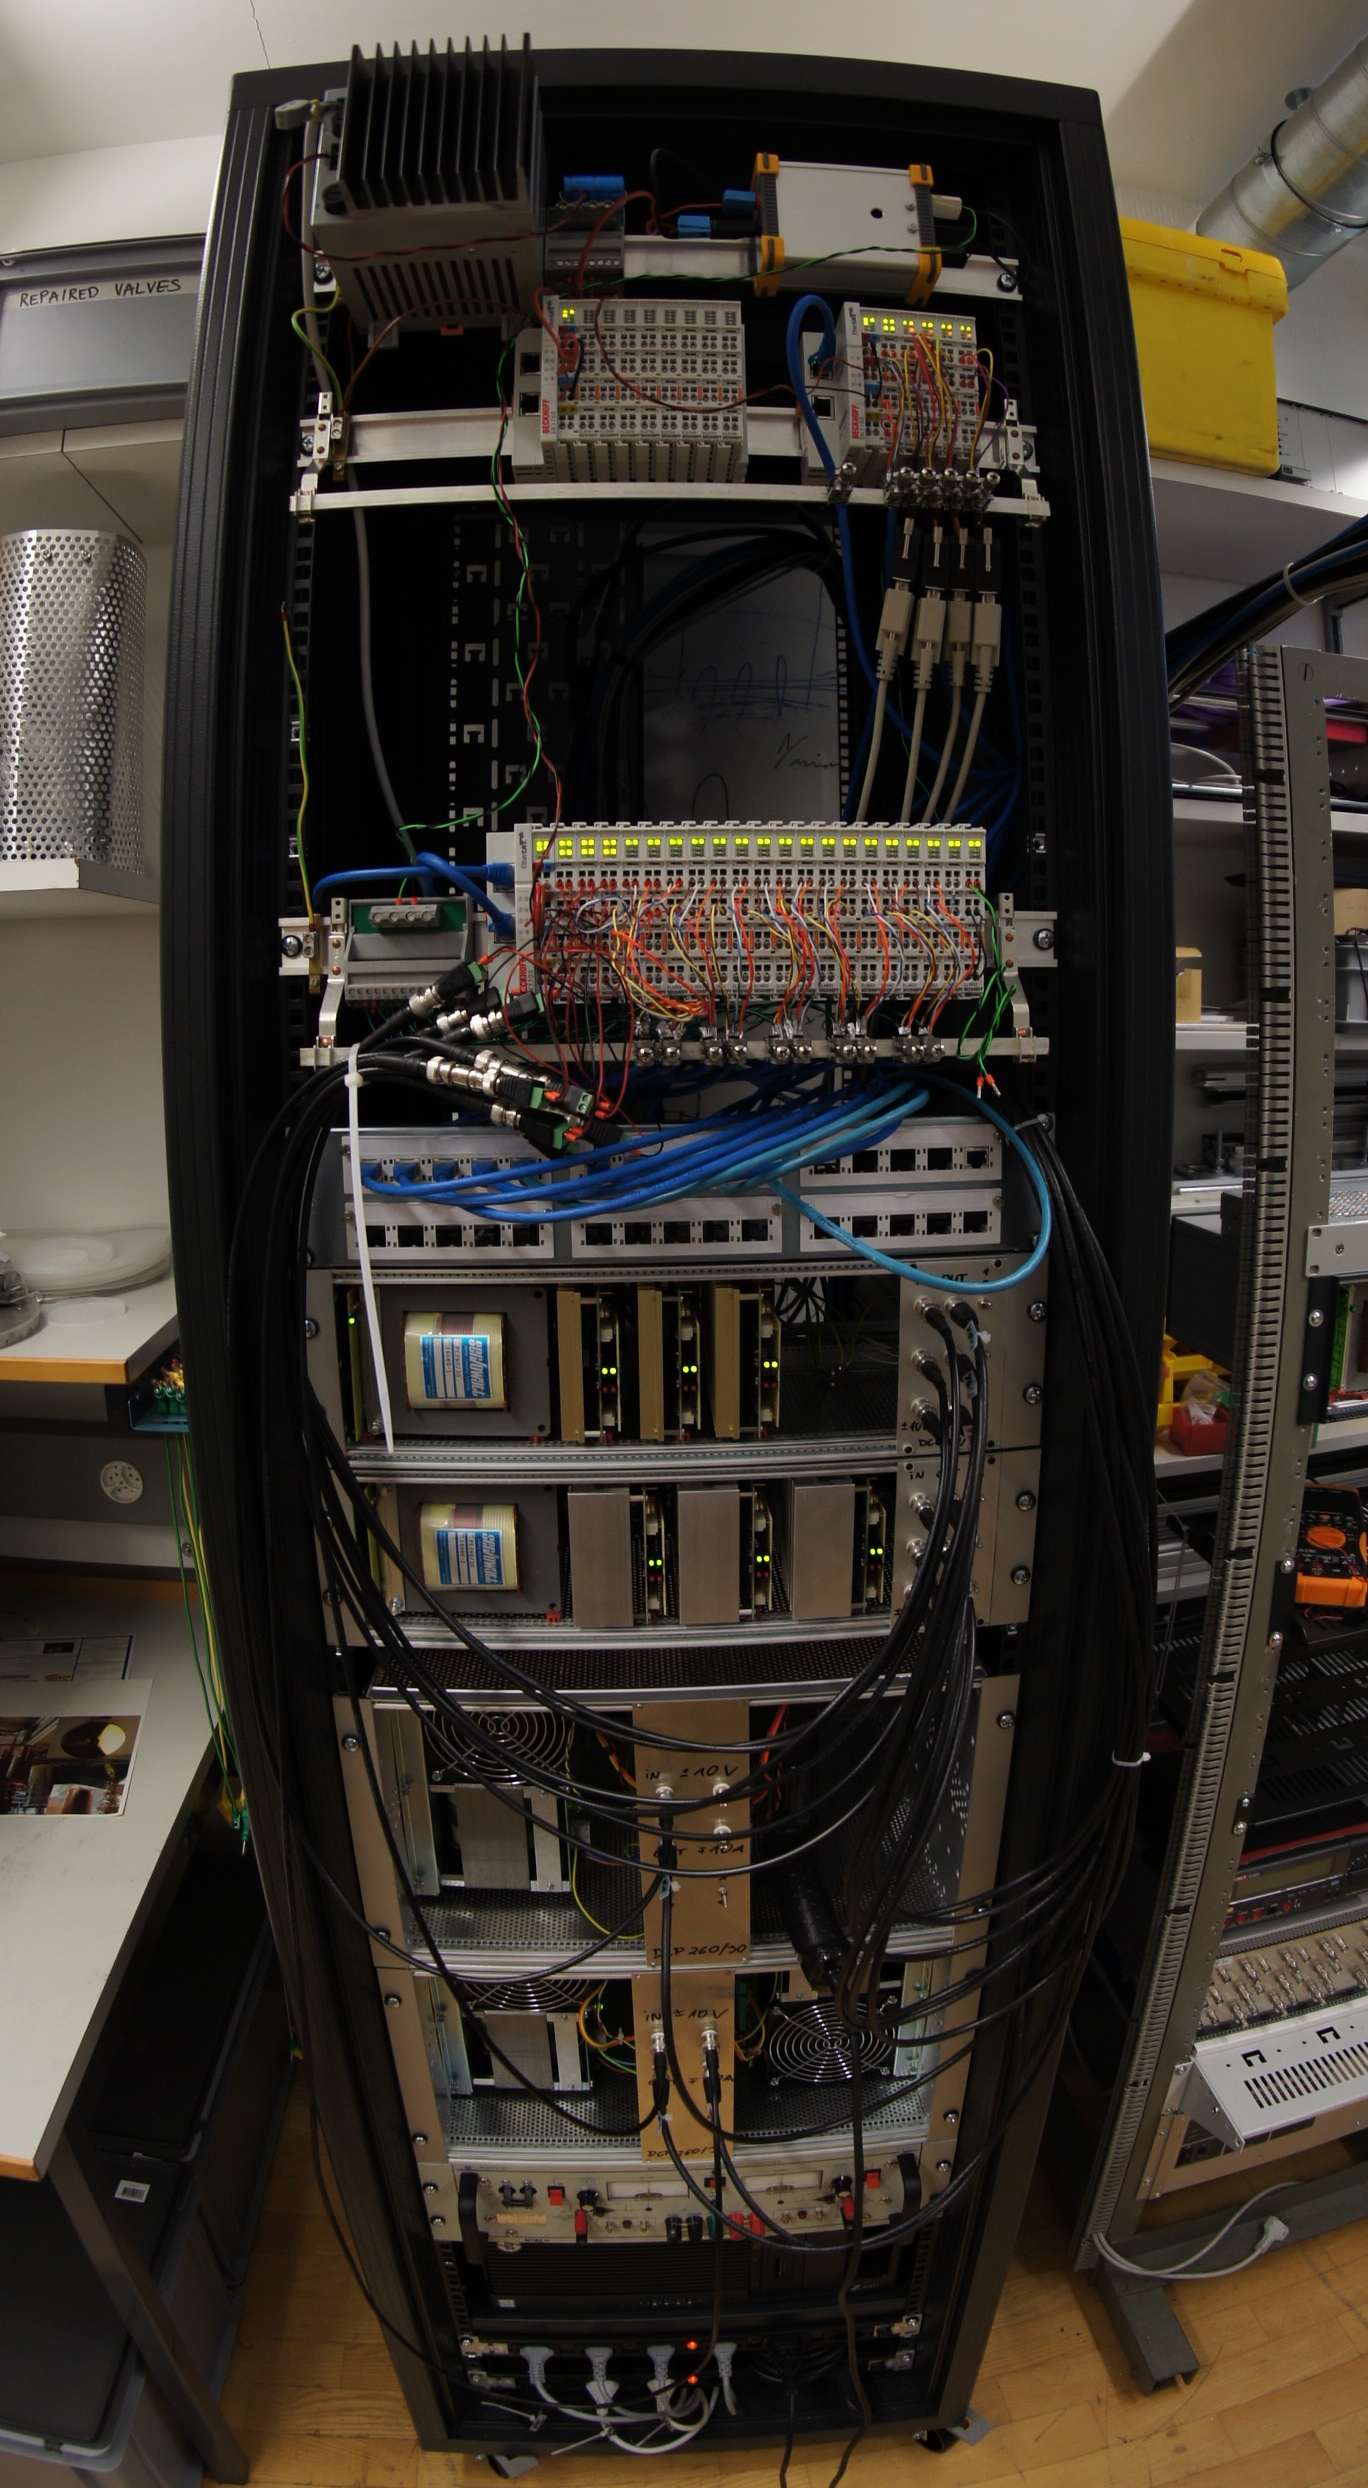
\includegraphics[width=0.6\linewidth,angle=90]{gfx/prototype/DSC03477.JPG}
  \caption{Mention, that it shows\ldots}
  \label{fig:prototype_photo_daq}
\end{figure}






\section{Open-design cage}

